\documentclass[12pt]{article}
\usepackage{amsmath}
\usepackage{graphicx}
\usepackage{float}
\usepackage{tabularx}
\begin{document}
\title{Lab 2 - Digitolling Time}
\author{Xin Gao}
\date{}
\maketitle

\section{Abstract}
We take input signals and digitally down convert them into low bandpass
filtered outputs. A given input signal is sampled in an
analog-to-digital converter to digitize it and then mixed with an
oscillation signal to get a desired sideband, whose waveform is filtered
in an form-malleable FIR filter to create a passband of allowed low
passbands. Such process is of great convenience to radio astronomy for
analyzing radio signals. 
\section{Introduction}
Whereas an analog signal sends information in the original, continuous
waveform, a digital signal sends information at discrete ranges. Many
electronic devices today, including computer processors, use digitized
signals because these signals provide exact values for the range at
specific times or frequencies. Waveforms in time domain is converted to
data in frequency domain via fourier transformation. In context of radio
astronomy, the goal is to process the received signals, which is
accomplished by a digital-down converter. Input signals can be naturally
high in frequency; for easier processing, a digital-down converter takes
a digitized intermediate-frequency signal, which results from a mixer
using a 'heterodyning' technique and filters out all but a low frequency
band 'centered' at 0, ultimately to allow our processor to
output the desired information relatively quickly.
\section{Methods and Procedure}
Our input to be bandpass-filtered for down conversion (in a FIR filter -
to be discussed later) is a digitally mixed signal. We begin our
procedure with examining the process of sampling, which is digitizing an
analog signal and is a process gated by criteria. Next we would examine
the results of mixing signals in a FPGA (discussed later). Finally, we
would design the workings of our FIR filter to put it all together for
down converting an input signal mixed with our local 'clock oscillator'. 
\subsection{Sampling and the Nyquist Criterion}
Sampled data can be interpreted in multiple ways. Of interest to us are
their waveform, especially in relation to Nyquist's Criterion (see
section below), and their power spectra, which is very useful for
analyzing the multiple frequency makeup for an input signal. Power
Spectrum can be derived using Fourier transformation.
\subsubsection{Waveform}
When sampling, we take the continuous, analog input signal and measure
its values at discrete time intervals to produce its digitized
version. The frequency $\nu_{s}$ at which we sample must be high enough
in order for the signal to be replicated accurately. For this
examination we use \textbf{20 MHz} as ths sample frequency. The maximum
signal frequency $\nu_{sig} = \nu_{max}$ that can be sampled correctly is 
known as the Nyquist frequency and obey the following criterion, known 
as the Nyquist's Criterion:
\begin{align}\nu_{s} = 2\nu_{max}\end{align}
Plot 1 of Figure 2 shows sampled data at Nyquist frequency. Frequencies
$\nu_{sig}$ above the Nyquist frequencies do not get sampled
properly but gets 'aliased' down to corresponding frequencies. Aliasing
is an effect when certain reconstructed signals from sampling become
indistinguishable from one another. Because $\nu_{s}$ is not high enough
to accurately reconstruct a signal at, for example, 0.8$\nu_{s}$, the
reconstructed signal will be similar to that of a lower frequency. It
turns out that aliased signals are symmetric about $\nu_{max}$; that is, 
the same frequency difference from $\nu_{max}$ (up to $\nu_{s}$) will produce
similar sampled data. For example, the sampled 0.8$\nu_{s}$ data would
look like the sampled 0.2 $\nu_{s}$. Mathematically, for the purpose of
sampling, it would not be a stretch to say:
\begin{align}\nu_{max} + \Delta{\nu} \approx \nu_{max} - \Delta{\nu} , \Delta{\nu}
  < \nu_{max}\end{align}
Figure 1 shows the result of sampling at different frequences below
$\nu_{s}$ not at $\nu_{max}$. Setting $\nu_{max}$ = $\nu_{s}$ and sampling would 
produce unfruitful results since the signal would get sampled once per 
wavelength, creating a 'direct current' looking output. Plot 2 of Figure
2 shows this result. Similar nonsensical results are obtained when
$\nu_{s} << \nu_{max}$ (see Figure 3).
\subsubsection{Power Spectrum}
The waveform we obtain from the signals is a time domain; that is, the
value (voltage in our case) at each point is a function of
time. We fourier transform this function, as defined by:
\begin{align}\hat{f}(\omega) = \int f(t) e^{-i\omega{t}} dt\end{align}
Here $\omega$ is frequency. Taking the fourier transform of a time domain
function outputs a frequency domain function. Since our single input
signal is of primarily one frequency value, we expect $f(\omega)$ to
contain a delta function, spiking at the input frequency. There are
actually two spikes at positive and negative $\nu_{sig}$. This occurence
arises from the complex nature of taking the fourier transform. This
makes sense mathematically taking into account the following identities:
\begin{align}e^{-i\omega{t}} = cos(-i\omega{t}) +
isin(-i\omega{t})\end{align}
\begin{align}cos(-i\omega{t}) = \frac{e^{-i\omega{t}}+e^{i\omega{t}}}{2}
  \\ isin(-i\omega{t}) =
  \frac{e^{-i\omega{t}}-e^{i\omega{t}}}{2}\end{align}
Since cosine is an even function, $cos(i\omega{t} = cos(-i\omega{t})$; the
transformation due to the complex cosine component mirrors the data at 0 
frequency and spawns the negative frequencies. The plots of Figure 4
show this phenomenon. These plots are called the power spectra of the
data from Figure 1. A power spectrum P can be obtained by taking the
square of the absolute value of the fourier transformed values:
\begin{align}S = |{\hat{f}(\omega)}|^2\end{align}
The power spectrum is power as a function of frequency; it describes the
amount of energy or power a given frequency has in our signal. As shown
in Figure 6 and plot 2 of Figure 5, $\nu_{sig}$ at or greater than or equal to $\nu_{s}$
produce 0-valued power spectra, which are physically unimportant. Plot
1 of Figure 5 shows the power spectrum for $\nu_{max}$. It peaks at its
expected frequency, but at and only at the negative side, interestingly. 
\subsection{Mixing Frequencies - Heterodyning}
Heterodyning is the process of combining two input signals to form
output signals. Typically, inputs of $\nu_{1}$ and $\nu_{2}$ will
produce both sum and difference outputs $\nu_{1} \pm \nu_{2}$. Signals
mix by an operation called convolution, or multiplication in the
fourier-transformed domain:
\begin{align}f(t)g(t) = f(t)\ast{g(t)} = \int
  \hat{f}{\omega}\hat{g}{\omega}e^{i\omega{t}}d\omega \end{align} 
Convolution is essentially the sliding of a signal over another one.The
two signals can be convolve analytically in an analog mixer such as
the ZAD-1 mini circuit or digitally in the ROACH (Reconfigurable Open
Architecture for Computer Hardware), which includes a FPGA (Field 
Programmable Gate Array), an analog-to-digital converter (in the FPGA), 
and a processor. 
\subsubsection{Mixing in the ZAD-1 and Fourier FIltering}
We start our mixing experiments with analog mixing using the ZAD-1 mini
circuit, which takes two input signals from the oscillators and 
outputs the data as array into our programs. For the frequencies of the
two signals, we use $\nu_{lo} = 1 MHz and \nu_{sig} = \nu_{lo} \pm
.05\nu_{lo}$. For the sake of sampling the Nyquist frequency, the sample
frequency chosen for each case is different. For $\nu_{sig} = \nu_{lo} -
.05\nu_{lo}$, $\nu_{sum} = 1.95 MHz$ so the sample frequency is \textbf{3.9
MHz}. For $\nu_{sig} = \nu_{lo} + .05\nu_{lo}$, $\nu_{sum} = 2.05 MHz$ so
the sample frequency is \textbf{4.1 MHz}. We use these values for our signals and
then take the power spectra of the output data from the
mixer. The power spectra for these two cases are plotted in Figure
7. Now, let's say, we would like
only one sideband so we can see the waveform due to only one real peak
value for the frequency; we would have to filter out the other one. This
can be accomplished by invoking the inverse fourier transform:
\begin{align}f(t) = \frac{1}{2\pi}\int f(\omega) e^{i\omega{t}} d\omega\end{align}
For relevance to radio astronomy, let's say we would like to keep the lower
sideband. We use one of our mixer outputs as the signal we'd like to
filter. Let's use $\nu_{sum} = 1.95 MHz$. Its waveform and fourier
transformed (not its power spectrum) data values  are plotted in Figure
8. We see four peaks as expected and we want to filter out all
frequencies values except those centered at the immediate positive and
negative lower sideband peaks. Since the fourier transform is a complex
operator, our data is a two-dimensional array so we must set both the
real and imaginary values to zero using our programs. After this is 
accomplished, we finally take the inverse fourier transformed data, 
which is plotted in Figure 9.
\subsubsection{Mixing in the ROACH and the SSB}
Whereas the previous experiments deals with sampling an mixed analog output,
this experiment deals with mixing digitized signals. We compare by
sending similar signals to the ones used for the analog mixer to the
analog-to-digital converter in the ROACH. The ROACH is connected with a 
oscillator 'clock' with an internal sample frequency of $\nu_{clock} =$ 200 MHz. For
this part we use 10 MHz for $\nu_{lo}$ and 9.5 MHz for $\nu_{sig}$. The
output data is stored in a BRAM (Block Random Access Memory) file in the
FPGA. We copy the data to our program and then mercilessly murder the
file from the FPGA so other processess can start running on it. The
power spectrum of the digitally mixed output is plotted in Figure 10; it
is similar to the result achieved from the analog mixing experiment. So
far, our power spectra are all double sidebanded (DSB); that is, they
contain all four peaks of the upper and lower sidebands. It is possible,
however, to obtain a single sidebanded power spectrum without using
filtering methods. We begin another mixing process with a signal of
$\nu_{sig} = 1 MHz$ and an oscillation from the clock. We use $\nu_{lo}
= \nu_{clock} * (64/256)$ as our frequency modulation. It is important
to have a factor that is a multiple of two in the numerator 2$\pi$ is
divided into 256 parts for each wavelength; if not for a factor of two,
our oscillator signal would be inaccurate and we would get a direct
current as the output. The sine and cosine components of $\nu_{lo}$ are
each mixed with $\nu_{sig}$. The power spectra of these two cases are
plotted in the first two plots of Figure 11. Finally, we add the
components together (by adding the array values in our program) and the
power spectrum result is shown in plot 3 of Figure 11. Unlike all the
other spectra, there are only two peaks! This is a single sideband power
spectrum. 
\subsection{FIR Filter}
Our ultimate goal is to experiment with digital down conversion. We want
our final output to be a low bandpass filtered equivalent of our input
mixed signal. Our filter, the finite impulse response filter, ideally, creates a
passband centered at 0 and 'abruptly' ends at a frequency cutoff, above
which no frequency is outputted. For this experiment we would like to
create a 5/8 bandpass filter; that is only 5/8 of our input frequency,
centered at 0, gets through. Let's take our input to run from -10
MHz to 10 MHz. For a 5/8 filtered result, we want the output to run
from -6.25 to 62.5 MHz. This would ideally appear as a rectangular
graph. To do so, we assign coefficients, which determines what the
job of the filter is and, to the filter. Since
multiplying in frequency domain is equivalent to convolving in time
domain, to get our filtered and convolved output signal, we simply
multiply, in frequency domain, our passband values by 1 and our stopband
values by 0. We first segment out frequency domain input into 8
parts. We operate on the FPGA and set the coefficients that corresponds
to each segment. Since the counter starts at 0 frequency towards the
positive end and then jump to the negative end, the values chosen for
those segments are are shown in Table 1. To get the time domain
coefficients, we use the inverse fourier transform on our data. 
\section{Data and Results}
Here are the plots from our experiments.
\subsection{Nyquist Criterion - Sampling Examples}
\begin{figure}[!htp]
\caption{Selected Sampled Signals for $f_{s} = 20 MHz$}
\centering
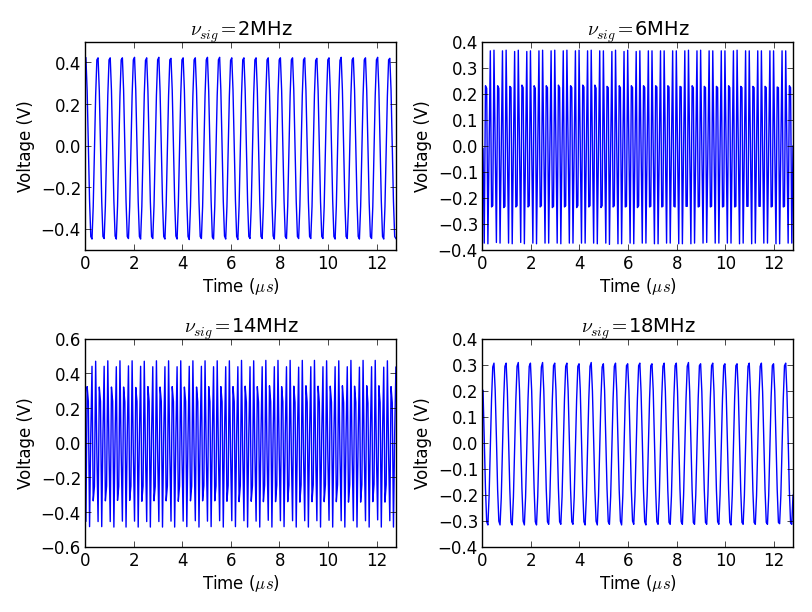
\includegraphics[width=.75\textwidth]{timesample1.png}\end{figure}
\begin{figure}[!hp]
\caption{Sampling at Nyquist Frequency and Sampling Frequency}
\centering
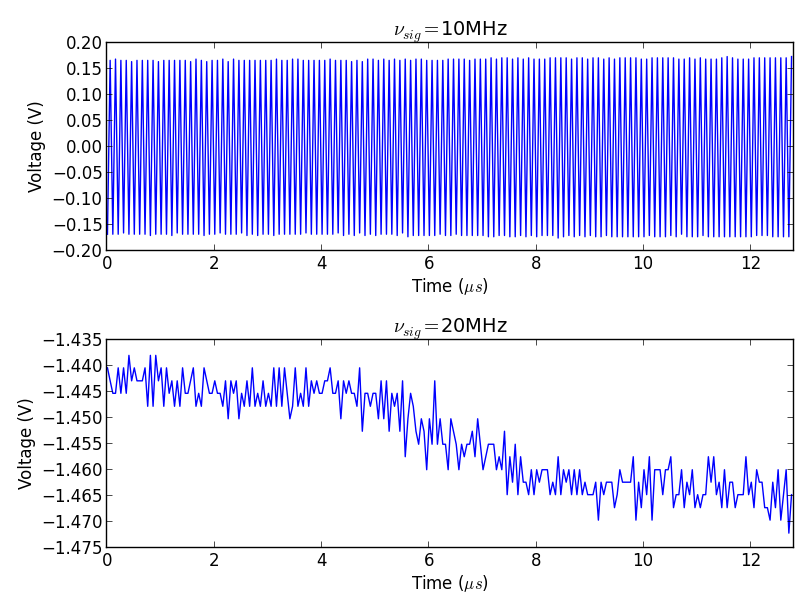
\includegraphics[width=.75\textwidth]{timesample2.png}\end{figure}
\begin{figure}[!hp]
\caption{The Nyquist Criterion Ignored}
\centering
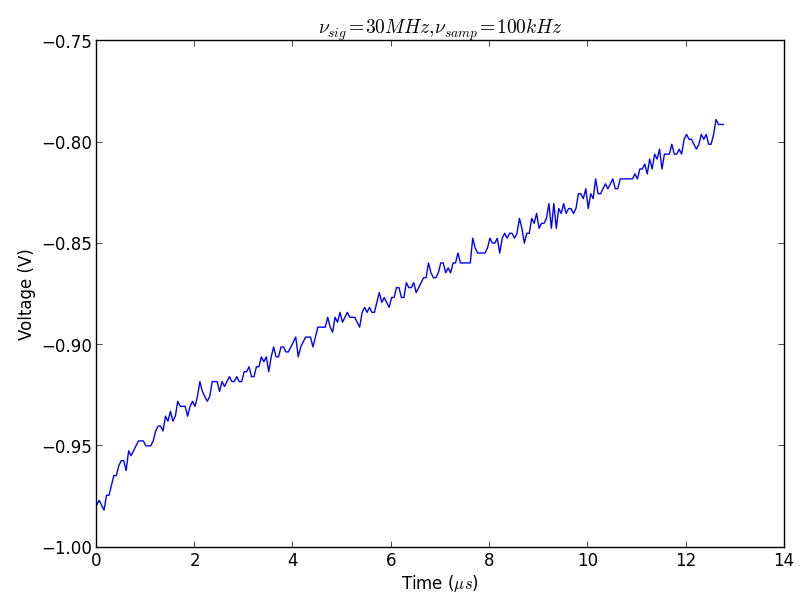
\includegraphics[width=.75\textwidth]{timesample3.png}\end{figure}
\begin{figure}[!hp]
\caption{Power Spectra Corresponding to Data from Figure 1}
\centering
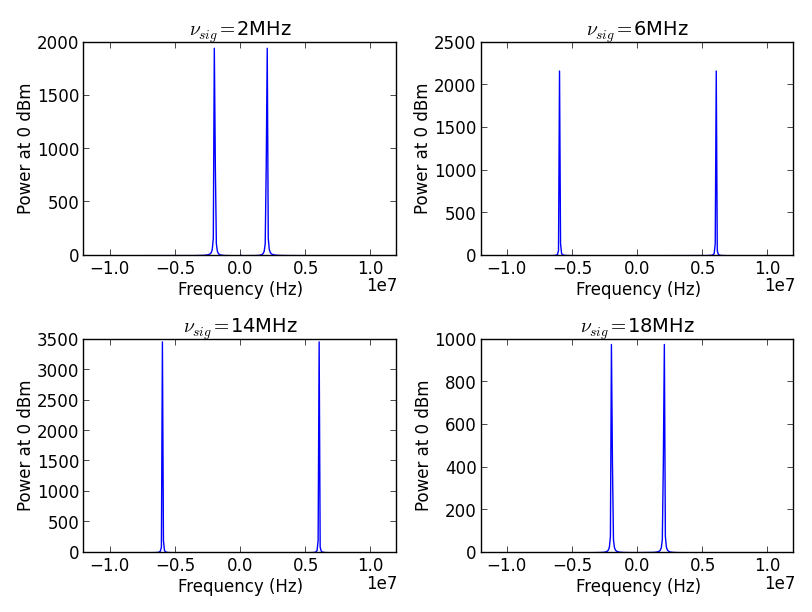
\includegraphics[width=.75\textwidth]{specsample1.png}\end{figure}
\begin{figure}[!hp]
\caption{Power Spectra Corresponding to Data from Figure 2}
\centering
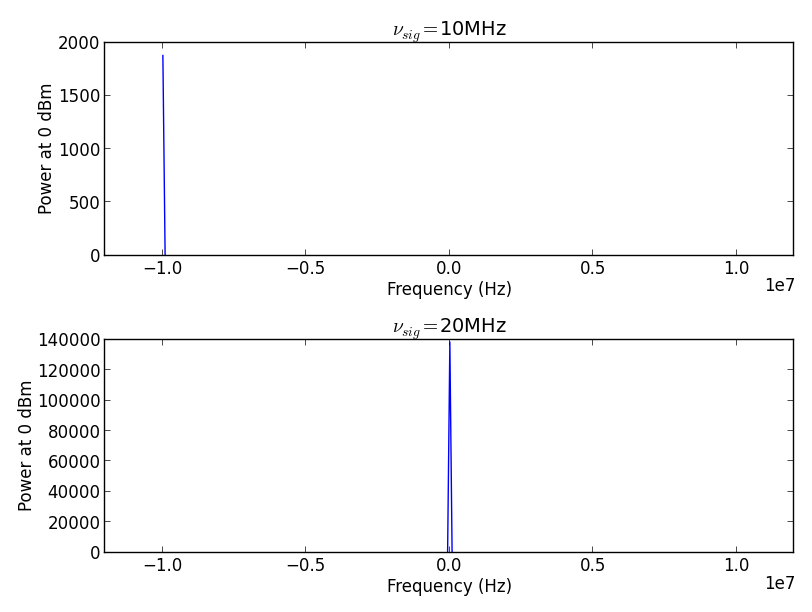
\includegraphics[width=.75\textwidth]{specsample2.png}\end{figure}
\begin{figure}[!hp]
\caption{Power Spectra Corresponding to Data from Figure 3}
\centering
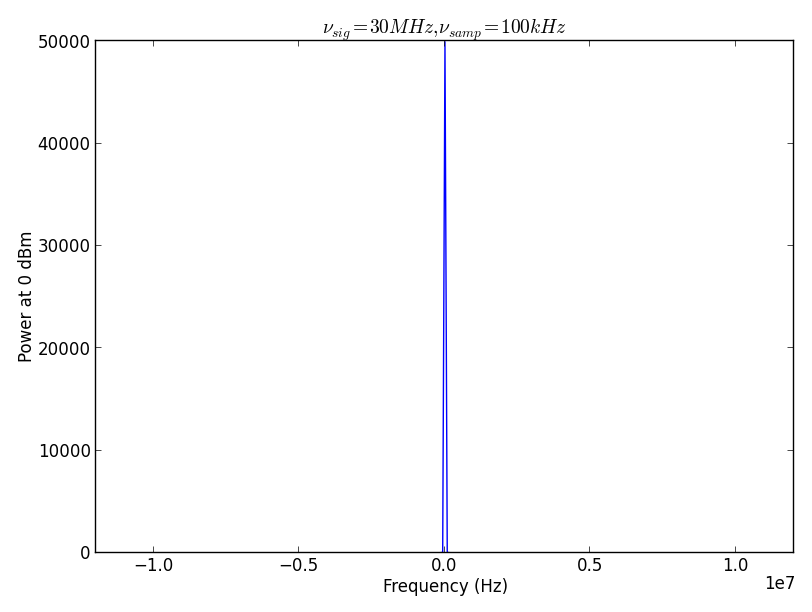
\includegraphics[width=.75\textwidth]{specsample3.png}\end{figure}
\newpage
\subsection{Analog Mixing}
\begin{figure}[!h]
\caption{Power Spectra of Analytically Mixed Signals}
\centering
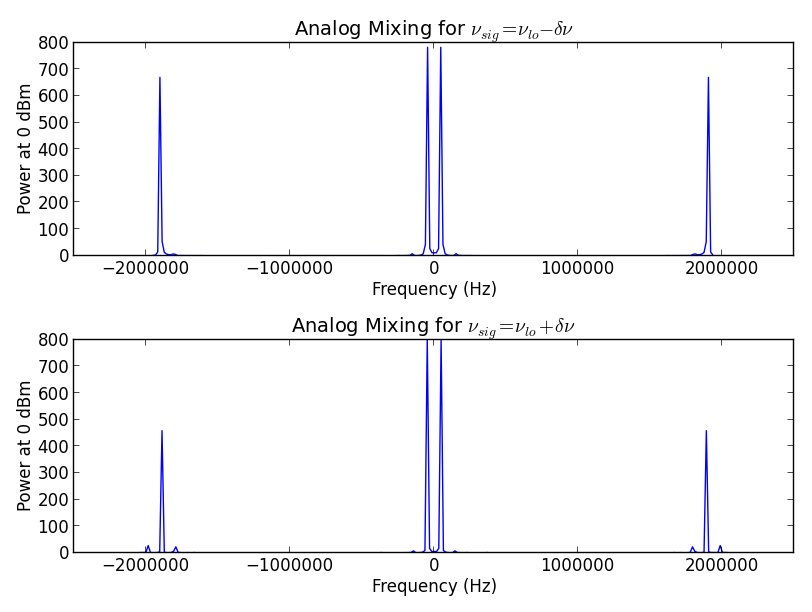
\includegraphics[width=.75\textwidth]{mixerspec.png}\end{figure}
\begin{figure}[!h]
\caption{Waveform and Fourier Transform of 1 ZAD-mixed Output}
\centering
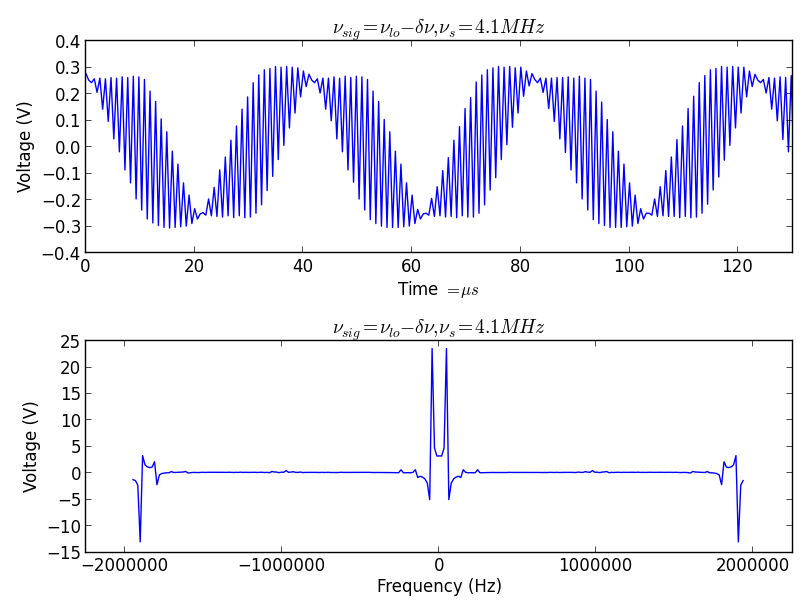
\includegraphics[width=.75\textwidth]{mixerwave.png}\end{figure}
\begin{figure}[!h]
\caption{Fourier-Filtered Waveform of Signal from Figure 8}
\centering
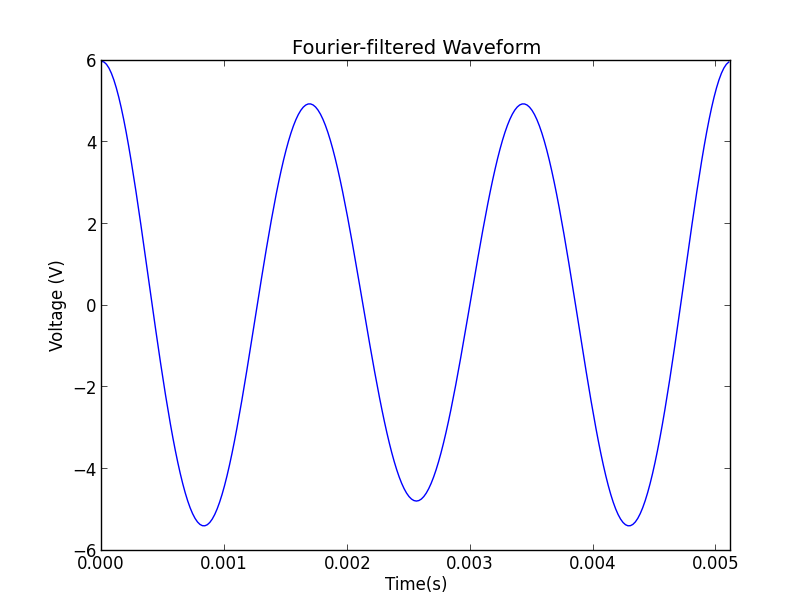
\includegraphics[width=.75\textwidth]{mixerfourier.png}\end{figure}
\newpage
\subsection{Digital Mixing: SSB vs. DSB}
\begin{figure}[!h]
\caption{Power Spectra of Digitally Mixed Signals}
\centering
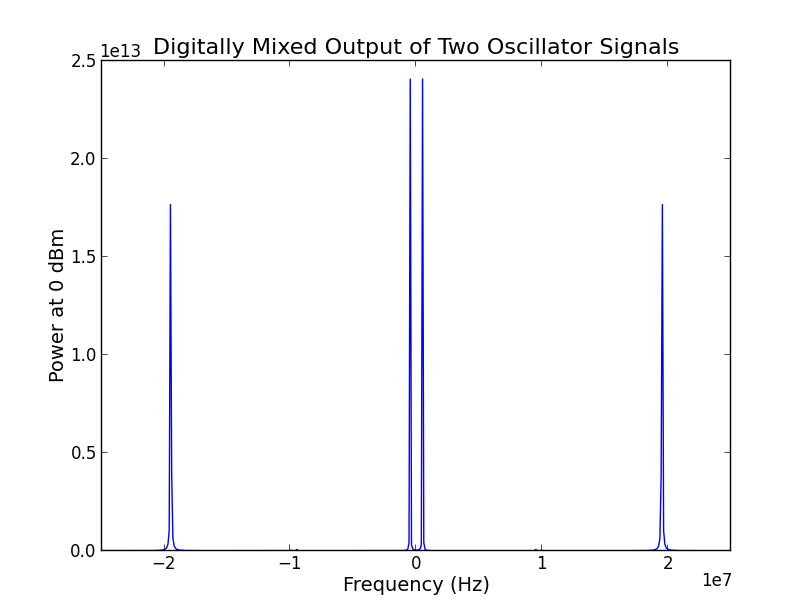
\includegraphics[width=.75\textwidth]{roachmix.png}\end{figure}
\begin{figure}[!h]
\caption{Power Spectra of Digitally Mixed Signals, SSB vs DSB Edition}
\centering
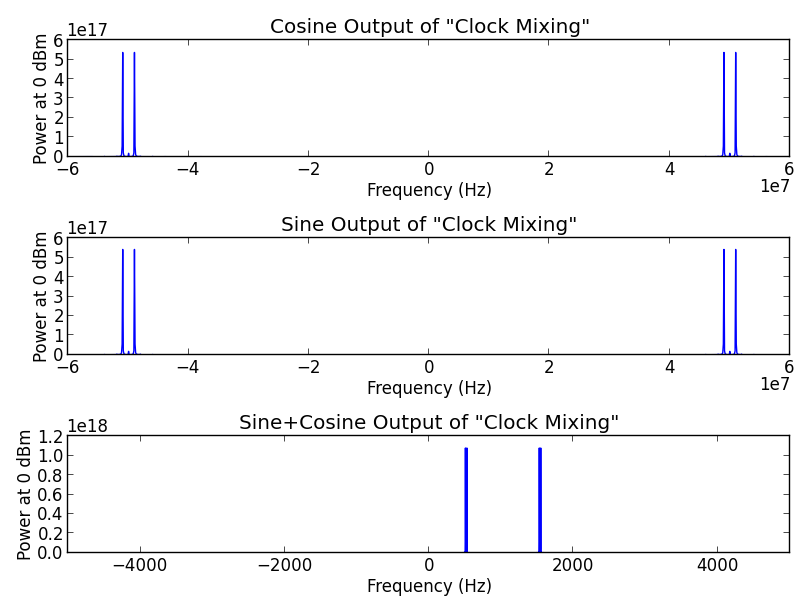
\includegraphics[width=.75\textwidth]{roachssb.png}\end{figure}
\newpage
\subsection{FIR Filter Coefficients}
\begin{table}[!h]
\caption{Coefficients for FIR Filter}
\centering
\begin{tabular}{c c c}
\hline\hline
N & coeff,realN & coeff,imagN \\ [0.5ex]
\hline 
0 & 1 & 1 \\
1 & 1 & 1 \\
2 & 1 & 1 \\
3 & 0 & 0 \\
4 & 0 & 0 \\
5 & 0 & 0 \\
6 & 1 & 1 \\
7 & 1 & 1 \\ [1ex]
\hline
\end{tabular}
\end{table}
\newpage
\section{Analysis and Discussion: The message of the Data}
What the plots convey is of paramount importance to the electronic world
surrounding us. Here we interpret that information that the our data
provide us with.
\subsection{Allies of Alias}
Figures 1 and 2 show the selected waveforms of $(N/10)\nu_{s}$ where N
is an integer from 1 to 10. Plot 1 of Figure 2 shows the highest
frequency because it is the waveform with Nyquist frequency $\nu_{max}$. The
waveform of this frequency is fully digitally represented by the
sampling frequency. The same goes for the lower frequencies shown in the
first two plots of Figure 1. For $\nu$ higher than $\nu_{max}$, the
sample frequency cannot accurately reconstruct the signal. The
reconstructed signal looks like one of a lower frequency; in fact, the
reconstructed waveforms' frequencies are symmetric about $\nu_{max}$, as
long as N is an integer between 0 and 10! This is the aliasing
phenomenon. A high $\nu_{sig}$ will 'alias down' to a lower
corresponding frequency. For frequencies at or above the sample
frequency, the reconstruction becomes very inaccurate and almost seems
noise-like. The result of approaching very relatively high frequencies
for $\nu_{sig}$ sseems to behave like a function of the first order, 
as shown in Figure 3. 
\subsection{Spectra of Power}
Figure 4 shows the peaks of the plots on either side of the symmetry
spreading farther apart (towards the value of the peak to $\nu_{max}$)
as $\nu_{sig}$ gets closer to $\nu_{max}$. Because of
aliasing, we expect the power spectrum of plot 4 to look like that of
plot 1 and the spectrum of plot 3 to look like that of plot 2, and they
do. The power spectrum of the Nyquist frequency has only 1 peak. This is
caused by the way the program plots Nyquist frequency samples: it begins
taking data at 0 and moves to positive values before jumping to the most
negative value and back to 0. Because sampling at the Nyquist frequency
outputs two peaks at the same frequency value corresponding to the
positive and negative 'edges', the program deems the two
indistinguishable; so, when it reaches the positive end, it jumps and
creates the peak value at the negative end. The power spectra for
$\nu_{sig} \geq \nu_{s}$ are 0 because the haphazard sampling for
relatively high frequencies produce meaningless reconstructions. 
\subsection{The Mixed Signals}
There seems to be four peaks total for each case in the analog mixing
experiment. They correspond to the sum and difference frequencies and
the complex mirror about 0. The sum frequency is known as the upper
sideband while the difference frequency is known as the lower
sideband. In radio signal analysis, the lower sideband is of special
importance for analysis. The digitally mixed result looks similar to our
analog result, as it should be. The digital result does look 'smoother,'
however. Mixing already digitized signals would create less
imperfections for the power spectrum because discrete mixing bypasses
many minor offsets cause my continuous mixing. There's also less
leakage, which arises from the nature of transforming into the frequency
domain from time domain. The waveform in time domain is primarily of
singular frequency, but there are also other, low-power and less
apparently frequencies mixed in. Frequency domain plots hence have
fluctuations at low power or voltage levels and this fluctuation can be
seen by taking the log scale of the power or voltage. 
\begin{figure}[!h]
\caption{Logarithmic Scale View in Frequency Domain - Leakage}
\centering
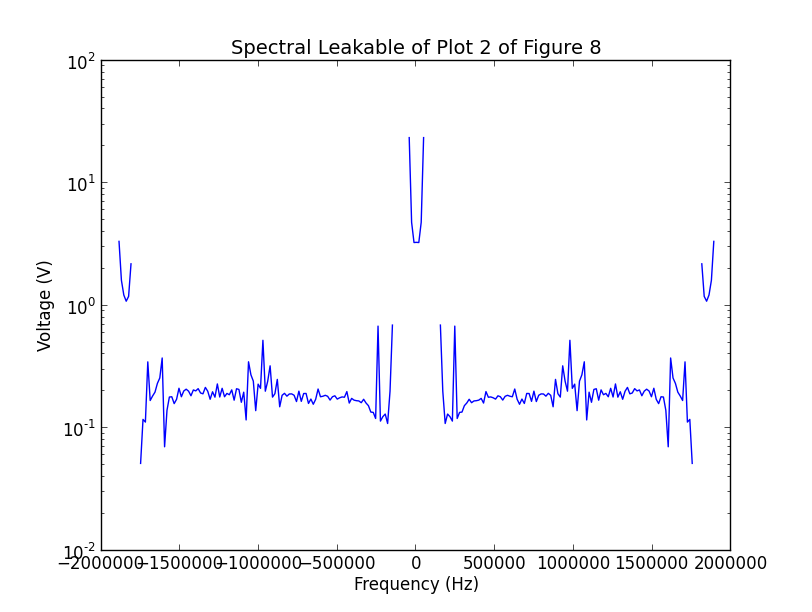
\includegraphics[width=.75\textwidth]{leakage.png}\end{figure}
This is not a very good representation of spectral leakage since this is
merely a voltage leakage from the fourier-transformed plot rather than a
power spectrum, but nonetheless presents the issue. Ideally, we would
like our graphs to have no leakage, but that is not what nature intends.
For our single sideband experiment, the sine and cosine components
combine to form a single sidebanded result. This arises from that our
program cannot normally distinguish positive and negative frequency 
values for representing them on a plot, but for this case, because sine 
and cosine have a phase difference, adding their arrays directly will
not 'mirror' the frequencies about 0. There are advantages to both
single and double sidebanded data. It comes down to what we would want:
to view both sidebands at once or only one, but a more noise-free one, 
at a time? This can be considered a quality versus quantity argument.
\subsection{FIR Filter Shape}
The FIR filter shape is dependent on the number of coefficients. For 8
coefficients, we expect a rather rectangular filter. As the number gets
greater, the filter is less 'digitized' and will deviate from a rigid
shape, displaying waveform like properties.
\section{Conclusion}
An input signal can be manipulated and analyzed in many ways to get
desired results. The goal of down converting a signal is significant in
our study of radio astronomy as it allows us to filter out unnecessary
high frequency components and analyze the low frequency band equivalent
of our signal. Methods of fourier transforming, sampling, and bandpass
filtering allows us to achieve our goal. From our input signal, the
information we extract includes how much power each present frequency
contributed to the signal - a very powerful (pun!) analysis.
\end{document}

